

\section{Methodology}
\begin{figure}[!tb]
    \centering
    % First Row
    \begin{minipage}{0.025\textwidth} % Narrow column for row label
        \raggedleft
        \rotatebox{90}{\text{RS}} % Vertical label for the first row
    \end{minipage}
    \begin{minipage}{0.06\textwidth}
        \centering
        
\includegraphics[width=\textwidth]{data_corrected/cam1_corrected/frame05.png}
        % \captionof{figure}{Rolling Shutter Image \(R_0\) where the corresponding Global Shutter image is at time \(t_0\)}

    \end{minipage}
    \begin{minipage}{0.06\textwidth}
        \centering
        
\includegraphics[width=\textwidth]{data_corrected/cam1_corrected/frame908.png}
        % \captionof{figure}{Rolling Shutter Image \(R_{N/2}\) where the corresponding Global Shutter image is at time \(t_{N/2}\)}
    \end{minipage}
    \begin{minipage}{0.06\textwidth}
        \centering
        
\includegraphics[width=\textwidth]{data_corrected/cam1_corrected/frame129.png}
        % \captionof{figure}{Rolling Shutter Image \(R_{N/2}\) where the corresponding Global Shutter image is at time \(t_{N/2}\)}
    \end{minipage}
    \begin{minipage}{0.06\textwidth}
        \centering
        
\includegraphics[width=\textwidth]{data_corrected/cam1_corrected/frame146.png}
        % \captionof{figure}{Rolling Shutter Image \(R_{N/2}\) where the corresponding Global Shutter image is at time \(t_{N/2}\)}
    \end{minipage}
    \begin{minipage}{0.06\textwidth}
        \centering
        
\includegraphics[width=\textwidth]{data_corrected/cam1_corrected/frame209.png}
        % \captionof{figure}{Rolling Shutter Image \(R_{N/2}\) where the corresponding Global Shutter image is at time \(t_{N/2}\)}
    \end{minipage}
    \begin{minipage}{0.06\textwidth}
        \centering
        
\includegraphics[width=\textwidth]{data_corrected/cam1_corrected/frame273.png}
        % \captionof{figure}{Rolling Shutter Image \(R_{N/2}\) where the corresponding Global Shutter image is at time \(t_{N/2}\)}
    \end{minipage}
    \begin{minipage}{0.06\textwidth}
        \centering
        
\includegraphics[width=\textwidth]{data_corrected/cam1_corrected/frame992.png}
        % \captionof{figure}{Rolling Shutter Image \(R_{N/2}\) where the corresponding Global Shutter image is at time \(t_{N/2}\)}
    \end{minipage}


    %second row
    \begin{minipage}{0.025\textwidth} % Narrow column for row label
        \raggedleft
        \rotatebox{90}{\text{GS}} % Vertical label for the first row
    \end{minipage}
       \begin{minipage}{0.06\textwidth}
        \centering
        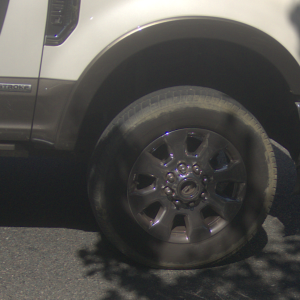
\includegraphics[width=\textwidth]{data_corrected/camera1/frame05.png}
        % \captionof{figure}{Rolling Shutter Image \(R_0\) where the corresponding Global Shutter image is at time \(t_0\)}

    \end{minipage}
    \begin{minipage}{0.06\textwidth}
        \centering
        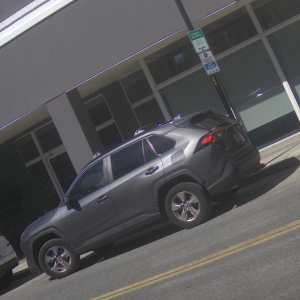
\includegraphics[width=\textwidth]{data_corrected/camera1/frame908.png}
        % \captionof{figure}{Rolling Shutter Image \(R_{N/2}\) where the corresponding Global Shutter image is at time \(t_{N/2}\)}
    \end{minipage}
    \begin{minipage}{0.06\textwidth}
        \centering
        
\includegraphics[width=\textwidth]{data_corrected/camera1/frame129.png}
        % \captionof{figure}{Rolling Shutter Image \(R_{N/2}\) where the corresponding Global Shutter image is at time \(t_{N/2}\)}
    \end{minipage}
    \begin{minipage}{0.06\textwidth}
        \centering
        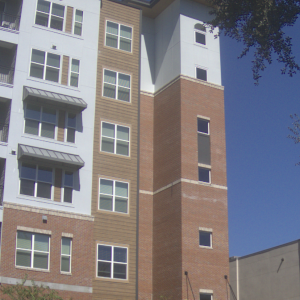
\includegraphics[width=\textwidth]{data_corrected/camera1/frame146.png}
        % \captionof{figure}{Rolling Shutter Image \(R_{N/2}\) where the corresponding Global Shutter image is at time \(t_{N/2}\)}
    \end{minipage}
    \begin{minipage}{0.06\textwidth}
        \centering
        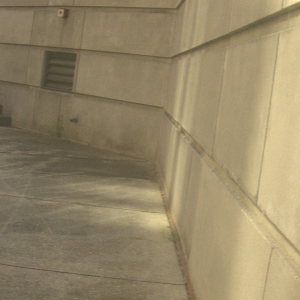
\includegraphics[width=\textwidth]{data_corrected/camera1/frame209.png}
        % \captionof{figure}{Rolling Shutter Image \(R_{N/2}\) where the corresponding Global Shutter image is at time \(t_{N/2}\)}
    \end{minipage}
    \begin{minipage}{0.06\textwidth}
        \centering
        
\includegraphics[width=\textwidth]{data_corrected/camera1/frame273.png}
        % \captionof{figure}{Rolling Shutter Image \(R_{N/2}\) where the corresponding Global Shutter image is at time \(t_{N/2}\)}
    \end{minipage}
    \begin{minipage}{0.06\textwidth}
        \centering
        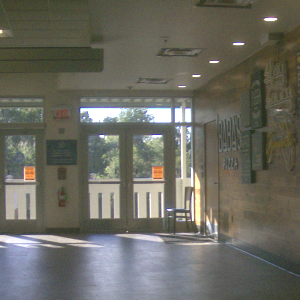
\includegraphics[width=\textwidth]{data_corrected/camera1/frame992.png}
        % \captionof{figure}{Rolling Shutter Image \(R_{N/2}\) where the corresponding Global Shutter image is at time \(t_{N/2}\)}
    \end{minipage}


    %Third Row
    \begin{minipage}{0.025\textwidth} % Narrow column for row label
        \raggedleft
        \rotatebox{90}{\text{RS}} % Vertical label for the first row
    \end{minipage}
       \begin{minipage}{0.06\textwidth}
        \centering
        
\includegraphics[width=\textwidth]{data_corrected/cam1_corrected/frame902.png}
        % \captionof{figure}{Rolling Shutter Image \(R_0\) where the corresponding Global Shutter image is at time \(t_0\)}

    \end{minipage}
    \begin{minipage}{0.06\textwidth}
        \centering
        
\includegraphics[width=\textwidth]{data_corrected/cam1_corrected/frame134.png}
        % \captionof{figure}{Rolling Shutter Image \(R_{N/2}\) where the corresponding Global Shutter image is at time \(t_{N/2}\)}
    \end{minipage}
    \begin{minipage}{0.06\textwidth}
        \centering
        
\includegraphics[width=\textwidth]{data_corrected/cam1_corrected/frame28.png}
        % \captionof{figure}{Rolling Shutter Image \(R_{N/2}\) where the corresponding Global Shutter image is at time \(t_{N/2}\)}
    \end{minipage}
    \begin{minipage}{0.06\textwidth}
        \centering
        
\includegraphics[width=\textwidth]{data_corrected/cam1_corrected/frame32.png}
        % \captionof{figure}{Rolling Shutter Image \(R_{N/2}\) where the corresponding Global Shutter image is at time \(t_{N/2}\)}
    \end{minipage}
    \begin{minipage}{0.06\textwidth}
        \centering
        
\includegraphics[width=\textwidth]{data_corrected/cam1_corrected/frame383.png}
        % \captionof{figure}{Rolling Shutter Image \(R_{N/2}\) where the corresponding Global Shutter image is at time \(t_{N/2}\)}
    \end{minipage}
    \begin{minipage}{0.06\textwidth}
        \centering
        
\includegraphics[width=\textwidth]{data_corrected/cam1_corrected/frame471.png}
        % \captionof{figure}{Rolling Shutter Image \(R_{N/2}\) where the corresponding Global Shutter image is at time \(t_{N/2}\)}
    \end{minipage}
    \begin{minipage}{0.06\textwidth}
        \centering
        
\includegraphics[width=\textwidth]{data_corrected/cam1_corrected/frame53.png}
        % \captionof{figure}{Rolling Shutter Image \(R_{N/2}\) where the corresponding Global Shutter image is at time \(t_{N/2}\)}
    \end{minipage}


    %fourth row
    \begin{minipage}{0.025\textwidth} % Narrow column for row label
        \raggedleft
        \rotatebox{90}{\text{GS}} % Vertical label for the first row
    \end{minipage}
   \begin{minipage}{0.06\textwidth}
        \centering
        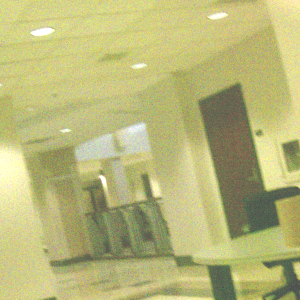
\includegraphics[width=\textwidth]{data_corrected/camera1/frame902.png}
        % \captionof{figure}{Rolling Shutter Image \(R_0\) where the corresponding Global Shutter image is at time \(t_0\)}

    \end{minipage}
    \begin{minipage}{0.06\textwidth}
        \centering
        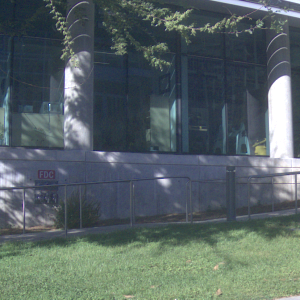
\includegraphics[width=\textwidth]{data_corrected/camera1/frame134.png}
        % \captionof{figure}{Rolling Shutter Image \(R_{N/2}\) where the corresponding Global Shutter image is at time \(t_{N/2}\)}
    \end{minipage}
    \begin{minipage}{0.06\textwidth}
        \centering
        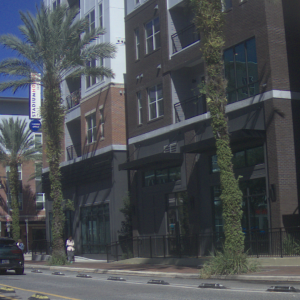
\includegraphics[width=\textwidth]{data_corrected/camera1/frame28.png}
        % \captionof{figure}{Rolling Shutter Image \(R_{N/2}\) where the corresponding Global Shutter image is at time \(t_{N/2}\)}
    \end{minipage}
    \begin{minipage}{0.06\textwidth}
        \centering
        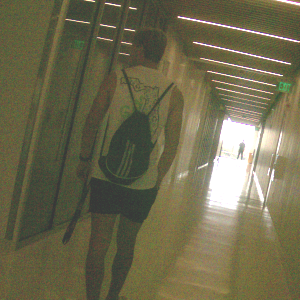
\includegraphics[width=\textwidth]{data_corrected/camera1/frame32.png}
        % \captionof{figure}{Rolling Shutter Image \(R_{N/2}\) where the corresponding Global Shutter image is at time \(t_{N/2}\)}
    \end{minipage}
    \begin{minipage}{0.06\textwidth}
        \centering
        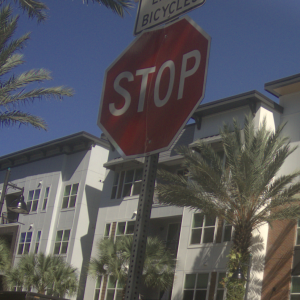
\includegraphics[width=\textwidth]{data_corrected/camera1/frame383.png}
        % \captionof{figure}{Rolling Shutter Image \(R_{N/2}\) where the corresponding Global Shutter image is at time \(t_{N/2}\)}
    \end{minipage}
    \begin{minipage}{0.06\textwidth}
        \centering
        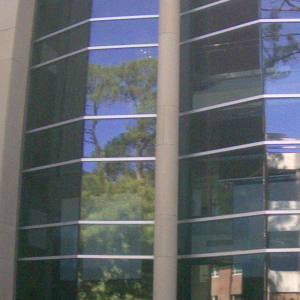
\includegraphics[width=\textwidth]{data_corrected/camera1/frame471.png}
        % \captionof{figure}{Rolling Shutter Image \(R_{N/2}\) where the corresponding Global Shutter image is at time \(t_{N/2}\)}
    \end{minipage}
    \begin{minipage}{0.06\textwidth}
        \centering
        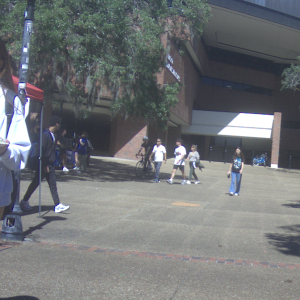
\includegraphics[width=\textwidth]{data_corrected/camera1/frame53.png}
        % \captionof{figure}{Rolling Shutter Image \(R_{N/2}\) where the corresponding Global Shutter image is at time \(t_{N/2}\)}
    \end{minipage}

    
    \caption{Highlights of the Real Dataset. Each pair of rows shows the rolling shutter capture and the corresponding global shutter capture. The dataset will be released to the public.}
    \label{fig:Real_Dataset}
    \vspace{-3mm}
\end{figure}

\subsection{Dataset Creation and Analysis}

To evaluate rolling shutter correction under large distortions, we provide three datasets containing paired RS and GS images. 

% These datasets emphasize motion profiles and distortions commonly encountered in robotic systems, and provide explicit anchor-point control for systematic study.

\vspace{1mm}
\noindent \textbf{SYN1: Synthetic Benchmark.}  
\textit{SYN1} contains RS–GS pairs rendered in Blender \cite{villar2021learning}. Each single-view scene (table fan, ceiling fan, propeller plane) includes two GS images for different anchor points and eight RS variants with increasing distortion, producing $(8 + 2)\times200 = 2000$ images per scene. 

% Randomization in lighting, colors, and textures ensures appearance diversity. To prevent overfitting, we hold out specific blade orientations (15° intervals) for testing.

\vspace{1mm}
\noindent \textbf{SYN2: Realistic RS Simulation.}  
\textit{SYN2} introduces realistic motions and textures while maintaining full control over RS effects. RS frames are synthesized from the high-speed X4K1000FPS dataset \cite{X4K} by row-wise stitching of consecutive GS frames. This method allows the selection of multiple anchor points for a single RS image.  The dataset includes \textbf{22{,}040} GS frames and \textbf{4{,}408} RS images, covering a variety of motions and scene types.

% Each RS image corresponds to five GS frames, defining five anchor points per sequence.

\noindent \textbf{REAL: Collocated RS-GS Capture.}
\textit{REAL} is a real-world dataset captured using a \textbf{dual-camera collocated system} (Fig.~\ref{fig:camera}), where rolling-shutter and global-shutter cameras are beam-splitter-aligned and hardware-synchronized. Varying trigger delays provides explicit control of the anchor point, producing multiple RS-GS pairs per scene. The dataset contains ~40k image pairs at 300×300 resolution (20k outdoor, 10k indoor, 10k additional for anchor point ablation). Optical-flow analysis (Fig.~\ref{fig:flow_bar}) shows that \textbf{REAL} exhibits the largest motion among RS datasets, making it suitable for evaluating large-distortion RS correction and depth estimation. 

% The system is attachable to a Puppy-Pi robot for legged-robot experiments
\begin{figure}[t!]
    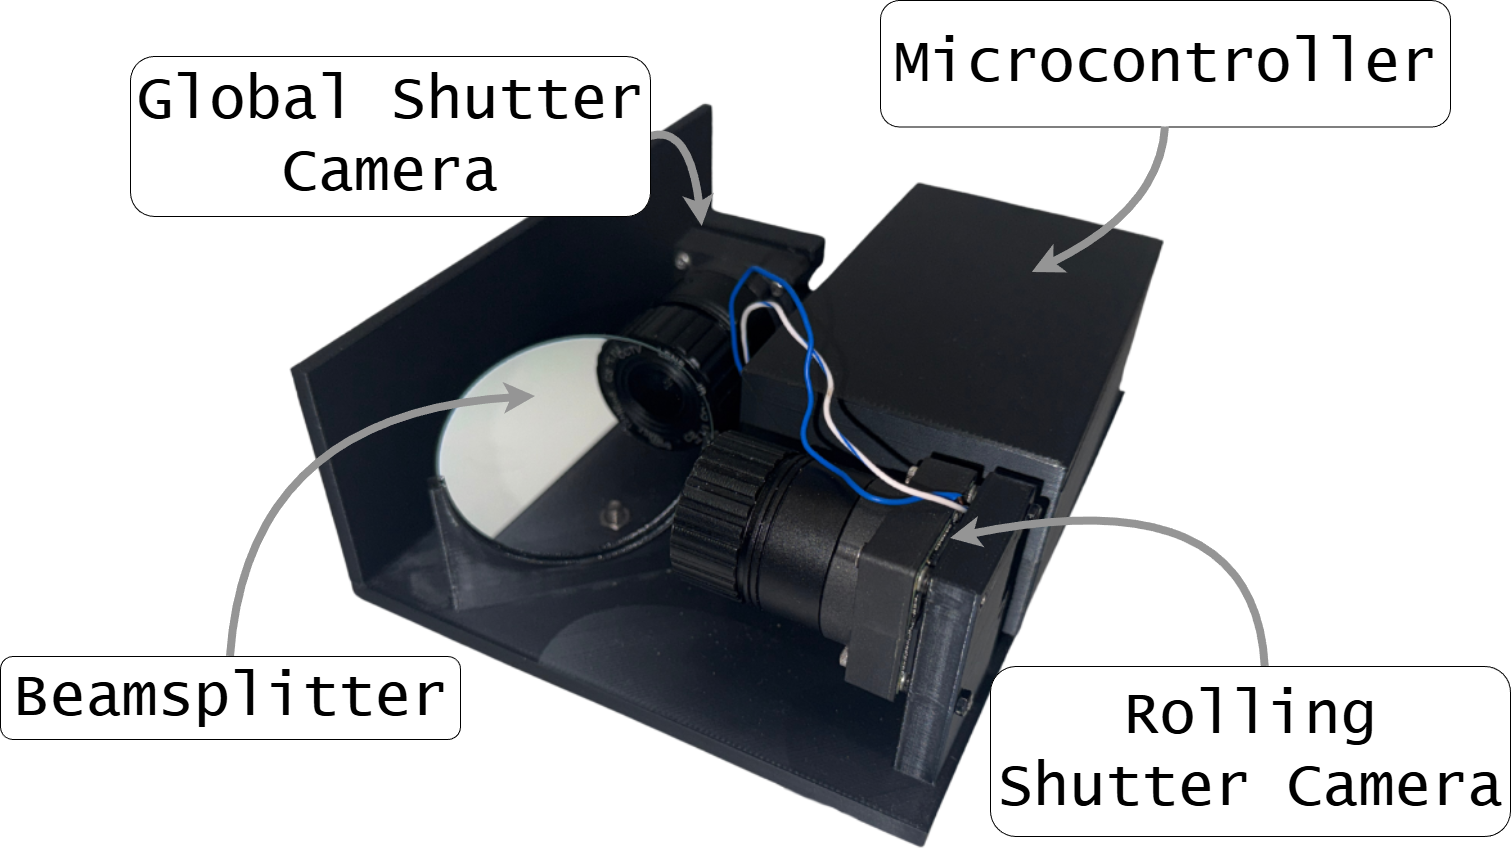
\includegraphics[width=0.55\columnwidth]{Figures/camera_diagram.drawio.png}
    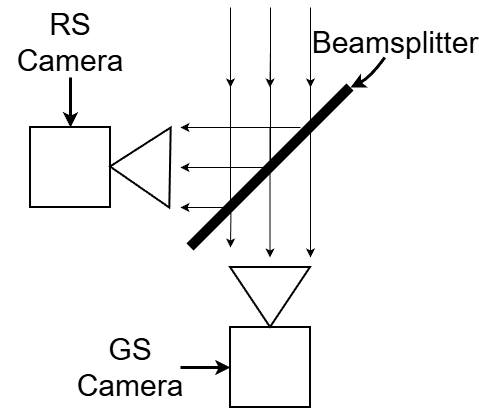
\includegraphics[width=0.4\columnwidth]{Figures/ray_diagram.drawio.png}
    \caption{Collocated RS–GS camera setup used for REAL. Hardware synchronization allows explicit control of anchor points for each capture. This device will be provided as a demo if accepted.}
    \label{fig:camera}
    \vspace{-2mm}
\end{figure}



\begin{figure*}[!bh]
    \centering

    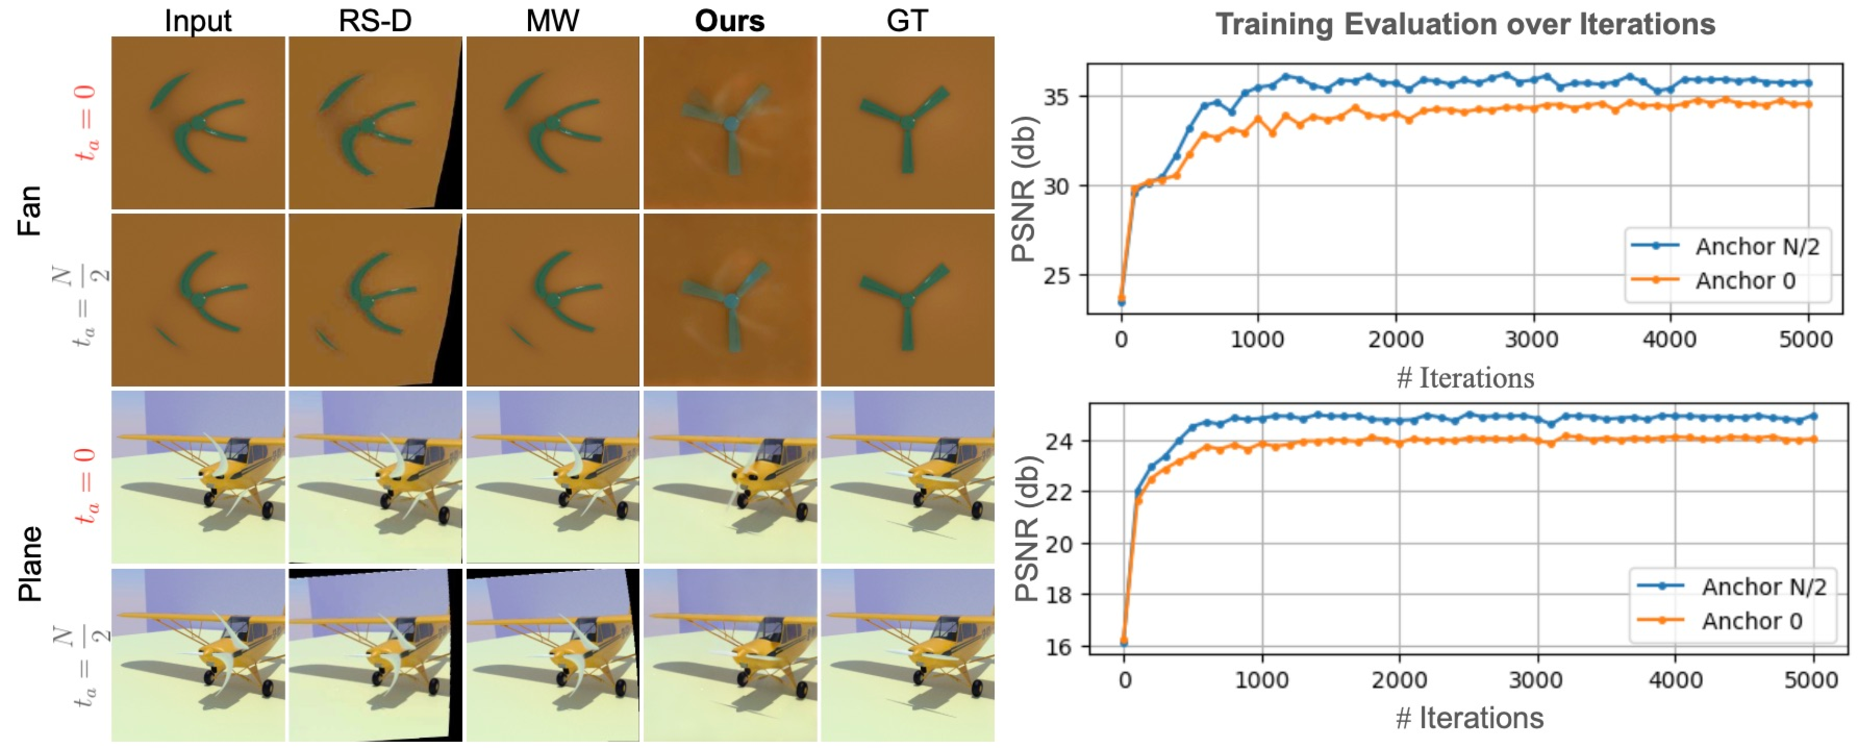
\includegraphics[width=\textwidth]{Results/SYNTH1.pdf}
    \caption{
    Results on SYN1 comparing RS-Diffusion \cite{RS-Diffusion}, Manhattan World \cite{Manhattan}, and our method under two anchor-point choices ($t_a=0$, $t_a=\frac{N}{2}$). PSNR curves show validation performance per anchor-point.
    % Visualization off our of the models run on synthetic data (\textbf{SYN1}). Each column corresponds to a method, and each row to a scene (Fan, Plane). Each scene shows the input with two anchors ($t_a=0$ and $t_a=\frac{N}{2}$), compared against RS-Diffusion \cite{RS-Diffusion}, Manhattan World \cite{Manhattan}, our model outputs, and ground truth. The PSNR curves on the right show training performance over iterations for each scene. %\JI{This figure needs a lot of revision}
    }
    \label{fig:rotated_fig_sidepsnr}
    \vspace{-4mm}
\end{figure*}
    % \begin{minipage}{0.6\textwidth} % LEFT: Images
    %     %---------------- Header Row ----------------%
    %     \hspace{.09\textwidth}
    %     \begin{minipage}{0.16\textwidth}\centering\textbf{Input}\end{minipage}
    %     \begin{minipage}{0.16\textwidth}\centering\textbf{RS-D} \cite{RS-Diffusion}\end{minipage}
    %     \begin{minipage}{0.16\textwidth}\centering\textbf{MW} \cite{Manhattan}\end{minipage}
    %     \begin{minipage}{0.16\textwidth}\centering\textbf{Ours}\end{minipage}
    %     \begin{minipage}{0.16\textwidth}\centering\textbf{GT}\end{minipage}

    %     \vspace{2mm}

    %     %---------------- FAN EXTREME ----------------%
    %     \begin{minipage}{0.02\textwidth}\rotatebox{90}{\textbf{Fan}}\end{minipage}
    %     \hspace{0.01\textwidth}
    %     \begin{minipage}{0.04\textwidth}
    %         \centering
    %         % \vspace{5mm}
    %         \rotatebox{90}{\textcolor{red}{$t_a = 0$}}\\[3mm]
    %         % \vspace{10mm}
    %         \rotatebox{90}{\textcolor{green}{$t_a = \frac{N}{2}$}}
    %     \end{minipage}
    %     \begin{minipage}{0.16\textwidth}\centering
    %         
\includegraphics[width=\textwidth]{Results/extreme/fan_extreme/start/0000.png}\\
    %         
\includegraphics[width=\textwidth]{Results/extreme/fan_extreme/center/0000.png}
    %     \end{minipage}
    %     \begin{minipage}{0.16\textwidth}\centering
    %         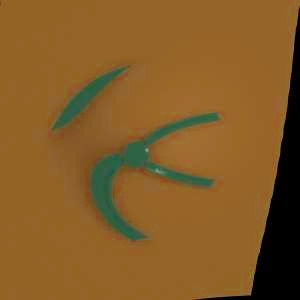
\includegraphics[width=\textwidth]{Results/RS-Diffusion/fs.jpg}\\
    %         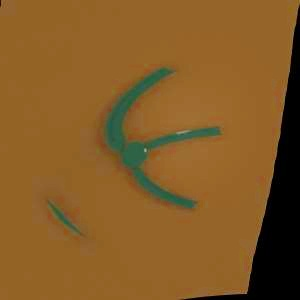
\includegraphics[width=\textwidth]{Results/RS-Diffusion/fc.jpg}
    %     \end{minipage}
    %     \begin{minipage}{0.16\textwidth}\centering
    %         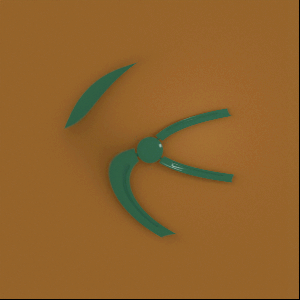
\includegraphics[width=\textwidth]{Results/manhattan/fs.png}\\
    %         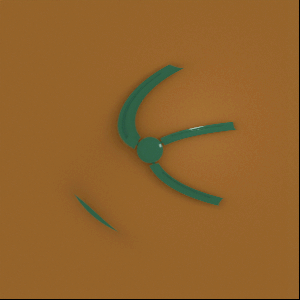
\includegraphics[width=\textwidth]{Results/manhattan/fc.png}
    %     \end{minipage}
    %     \begin{minipage}{0.16\textwidth}\centering
    %         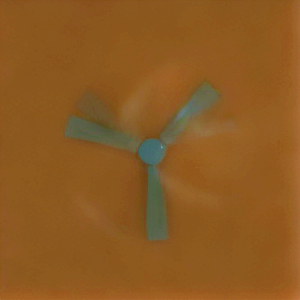
\includegraphics[width=\textwidth]{Results/extreme/fan_extreme/start/fan_extreme_test_RS0.8_START_0000.png}\\
    %         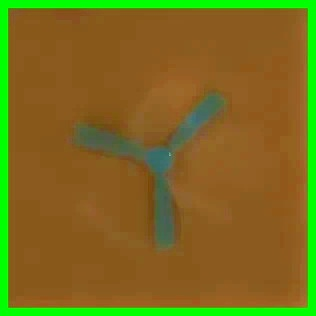
\includegraphics[width=\textwidth]{Results/extreme/fan_extreme/center/0000_green.jpg}
    %     \end{minipage}
    %     \begin{minipage}{0.16\textwidth}\centering
    %         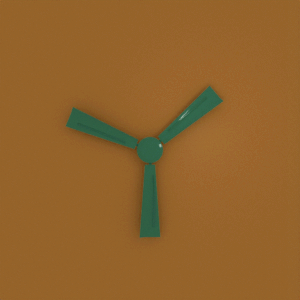
\includegraphics[width=\textwidth]{Results/extreme/fan_extreme/0000.png}\\
    %         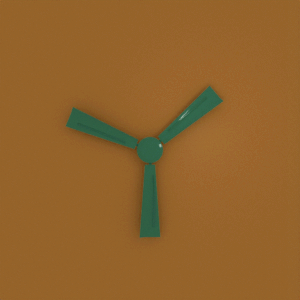
\includegraphics[width=\textwidth]{Results/extreme/fan_extreme/0000.png}
    %     \end{minipage}
    %     \vspace{0mm}
        
    %     %---------------- PLANE EXTREME ----------------%
    %     \begin{minipage}{0.02\textwidth}\rotatebox{90}{\textbf{Plane}}\end{minipage}
    %     \hspace{0.01\textwidth}
    %     \begin{minipage}{0.04\textwidth}
    %         \centering
    %         \vspace{5mm}
    %         \rotatebox{90}{\textcolor{red}{$t_a = 0$}}\\[3mm]
    %         % \vspace{13mm}
    %         \rotatebox{90}{\textcolor{green}{$t_a = \frac{N}{2}$}}
    %     \end{minipage}
    %     \begin{minipage}{0.16\textwidth}\centering
    %         
\includegraphics[width=\textwidth]{Results/extreme/plane_extreme/start/0000.png}\\
    %         
\includegraphics[width=\textwidth]{Results/extreme/plane_extreme/center/0000.png}
    %     \end{minipage}
    %     \begin{minipage}{0.16\textwidth}\centering
    %         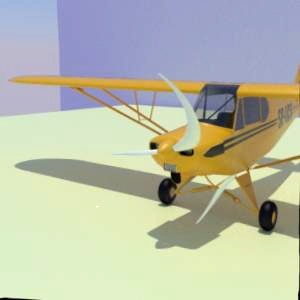
\includegraphics[width=\textwidth]{Results/RS-Diffusion/ps.jpg}\\
    %         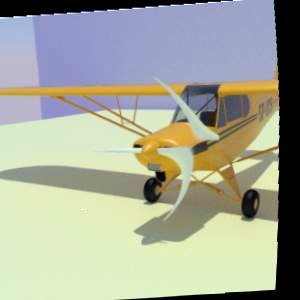
\includegraphics[width=\textwidth]{Results/RS-Diffusion/pc.jpg}
    %     \end{minipage}
    %     \begin{minipage}{0.16\textwidth}\centering
    %         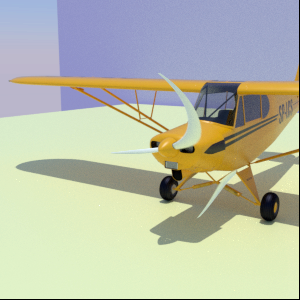
\includegraphics[width=\textwidth]{Results/manhattan/ps.png}\\
    %         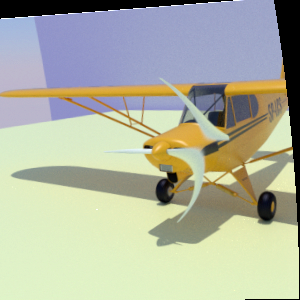
\includegraphics[width=\textwidth]{Results/manhattan/pc.png}
    %     \end{minipage}
    %     \begin{minipage}{0.16\textwidth}\centering
    %         
\includegraphics[width=\textwidth]{Results/extreme/plane_extreme/start/0000_pred.png}\\
    %         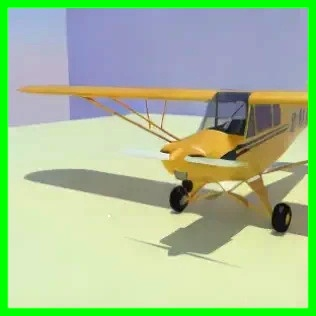
\includegraphics[width=\textwidth]{Results/extreme/plane_extreme/center/0000_pred_green.jpg}
    %     \end{minipage}
    %     \begin{minipage}{0.16\textwidth}\centering
    %         
\includegraphics[width=\textwidth]{Results/extreme/plane_extreme/0000.png}\\
    %         
\includegraphics[width=\textwidth]{Results/extreme/plane_extreme/0000.png}
    %     \end{minipage}
    % \end{minipage}%
    % % \hfill
    % \begin{minipage}{0.4\textwidth} % RIGHT: PSNR plots
    %     \centering
    %     \vspace{5mm}
    %     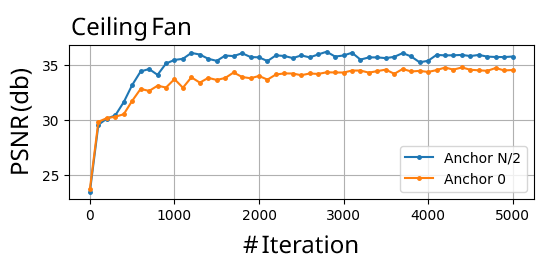
\includegraphics[width=\textwidth]{Results/fan/fan_psnr.png}\\
    %     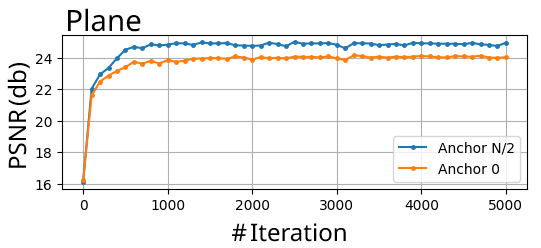
\includegraphics[width=\textwidth]{Results/Plane/plane_psnr.png}
    % \end{minipage}




\begin{figure}[t!]
    \centering
    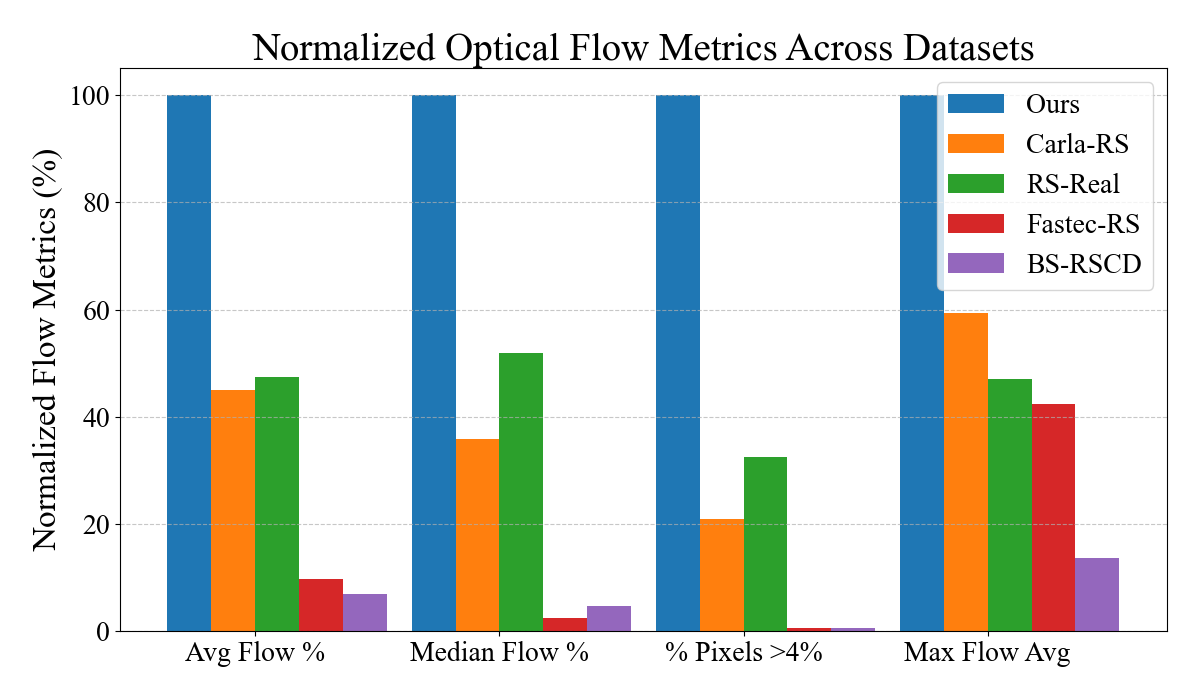
\includegraphics[width=\columnwidth]{collage/Figure_1.png}%
    \vspace{-2mm}
    \caption{Optical-flow motion statistics for RS datasets. For our dataset, the percentage of pixels with greater than 2\%, 6\%, and 10\% flow was more than double that of the other datasets. \textbf{No other dataset matches our egocentric motion, allowing us to model legged robots and other mobile systems.}}
    \label{fig:flow_bar}
    \vspace{-2mm}
\end{figure}





\subsection{Integration of Vision Foundation Models}

To address RS correction and monocular depth estimation, we leverage pre-existing vision foundation models (VFMs). Our pipeline consists of two sequential stages:




\begin{enumerate}
    \item \textbf{RS Correction Stage:} We adopt a Marigold U-Net~\cite{StableDiffusion} trained to map RS images to corresponding GS frames. The model operates on RGB images and focuses on removing row-wise distortions while preserving structure.
    
    \item \textbf{Monocular Depth Estimation Stage:} Corrected RS frames from the first stage are passed to a transformer-based Depth-Anything-V2~\cite{DepthAnything}. This stage produces dense depth maps, benefiting from the reduction in RS-induced geometric distortions. 
\end{enumerate}
\draft{Since metric depth ground truth is unavailable for the RS-GS datasets, we evaluate depth consistency relative to a frozen Depth-Anything-V2 teacher operating on the GS image. This measures preservation of geometric structure after RS correction rather than absolute metric depth accuracy. The teacher provides a consistent reference across all methods, isolating errors introduced by rolling shutter distortions.
}

\noindent \textbf{Pipeline Details.}  
The stages are trained sequentially: first, the Marigold U-Net is trained for RS correction; second, the corrected outputs are used to  fine-tune the depth model. 

% We experimented with different VFM configurations and found that sequentially applying two distinct VFMs yields better depth accuracy than either model alone. 

\vspace{1mm}
\noindent \textbf{Training Setup.}  
Both stages are trained using our RS-GS paired datasets (\textbf{SYN1}, \textbf{SYN2}, \textbf{REAL}). Standard image augmentation is applied, and losses include MSE loss for RS correction and scale invariant loss for Depth-Anything-V2. 

% All other architectural components (e.g., U-Net layers, transformer blocks) remain unchanged from the original VFMs, highlighting that improvements derive from task-specific training and anchor-point alignment.

% \vspace{1mm}
% \noindent \textbf{Purpose of VFM Integration.}  
% We use Vision Foundation Models (VFMs) to leverage strong priors for RGB reconstruction and monocular depth estimation, allowing us to isolate and analyze rolling shutter distortions and anchor-point effects. Depth-Anything is employed as a second-stage evaluator to assess structural and geometric consistency of the corrected outputs, rather than focusing on high-frequency photometric artifacts. This enables evaluation of rolling shutter behavior at a geometric level relevant to depth estimation.

\draft{\subsection{Comparisons and Baselines}
All trainable baselines were fine-tuned on the training splits used by our method whenever training code and model weights were publicly available \cite{RS-Diffusion}. For methods whose temporal reference is fixed by design, results are reported using the authors' original formulation. Evaluation was performed on identical testing data. Baselines of the author's original implementations are included alongside fine-tuned implementations.
}
% \begin{figure*}[t!]
%     \vspace{2mm}  % vertical space + line break
%     \centering
% \parbox{0.04\textwidth}{\centering {}}
% \parbox{0.095\textwidth}{\centering \textbf{SYN2}}
% \rule{0.6pt}{.3cm}
% \parbox{0.725\textwidth}{\centering \textbf{REAL / RS-GS}}


    
%     % Input Image
%     \begin{minipage}{0.05\textwidth} % Narrow column for row label
%         \raggedleft
%         \rotatebox{90}{\text{Input Image}} % Vertical label for the first row
%     \end{minipage}
%     \begin{minipage}{0.115\textwidth}
%         \vspace{0.05cm}
%         \centering
%         
\includegraphics[width=\textwidth]{X4K_data/input/occ068.802_f3921.png}
%     \end{minipage}
%     \begin{minipage}{0.115\textwidth}
%         \vspace{0.05cm}
%         \centering
%         
\includegraphics[width=\textwidth]{Collocated_Collage/input/frame08.png}
%     \end{minipage}
%     \begin{minipage}{0.115\textwidth}
%         \vspace{0.05cm}
%         \centering
%         
\includegraphics[width=\textwidth]{Collocated_Collage/10-20-vis/input/frame184.png}
%     \end{minipage}
%     \begin{minipage}{0.115\textwidth}
%         \vspace{0.05cm}
%         \centering
%         
\includegraphics[width=\textwidth]{Collocated_Collage/input/frame958.png}
%     \end{minipage}
%     \begin{minipage}{0.115\textwidth}
%         \vspace{0.05cm}
%         \centering
%         
\includegraphics[width=\textwidth]{Collocated_Collage/10-20-vis/input/frame264.png}
%     \end{minipage}
%     \begin{minipage}{0.115\textwidth}
%         \vspace{0.05cm}
%         \centering
%         
\includegraphics[width=\textwidth]{Collocated_Collage/input/frame96.png}
%     \end{minipage}
%     \begin{minipage}{0.115\textwidth}
%         \vspace{0.05cm}
%         \centering
%         
\includegraphics[width=\textwidth]{Collocated_Collage/10-20-vis/input/frame691.png}
%     \end{minipage}
%     \hspace{0.05\textwidth}

%     % Manhattan
%     \begin{minipage}{0.05\textwidth} % Narrow column for row label
%         \raggedleft
%         \rotatebox{90}{\text{MW \cite{Manhattan}}} % Vertical label for the first row
%     \end{minipage}
%     \begin{minipage}{0.115\textwidth}
%         \vspace{0.05cm}
%         \centering
%         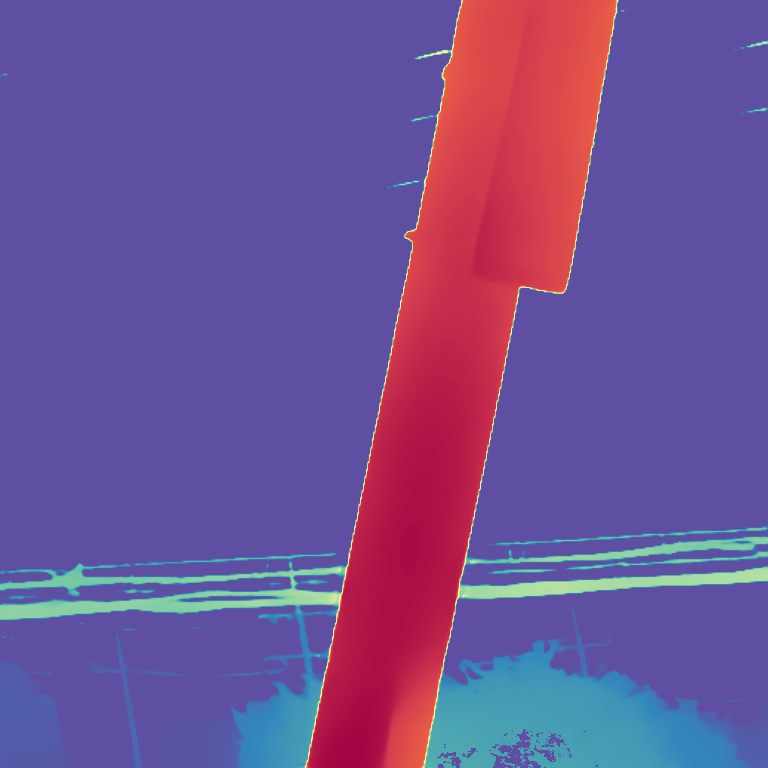
\includegraphics[width=\textwidth]{Collocated_Collage/mw_depth/manhattan_world/068mw.png}
%     \end{minipage}
%     \begin{minipage}{0.115\textwidth}
%         \vspace{0.05cm}
%         \centering
%         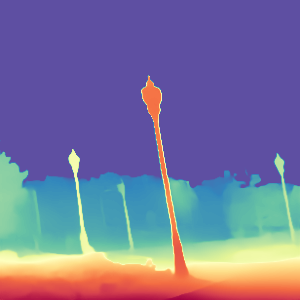
\includegraphics[width=\textwidth]{Collocated_Collage/mw_depth/output_frame08.png}
%     \end{minipage}
%     \begin{minipage}{0.115\textwidth}
%         \vspace{0.05cm}
%         \centering
%         
\includegraphics[width=\textwidth]{Collocated_Collage/mw_depth/manhattan_world/frame184mw.png}
%     \end{minipage}
%     \begin{minipage}{0.115\textwidth}
%         \vspace{0.05cm}
%         \centering
%         
\includegraphics[width=\textwidth]{Collocated_Collage/mw_depth/output_frame958.png}
%     \end{minipage}
%     \begin{minipage}{0.115\textwidth}
%         \vspace{0.05cm}
%         \centering
%         
\includegraphics[width=\textwidth]{Collocated_Collage/mw_depth/manhattan_world/frame264mw.png}
%     \end{minipage}
%     \begin{minipage}{0.115\textwidth}
%         \vspace{0.05cm}
%         \centering
%         
\includegraphics[width=\textwidth]{Collocated_Collage/mw_depth/manhattan_world/frame96mw.png}
%     \end{minipage}
%     \begin{minipage}{0.115\textwidth}
%         \vspace{0.05cm}
%         \centering
%         
\includegraphics[width=\textwidth]{Collocated_Collage/mw_depth/manhattan_world/frame691mw.png}
%     \end{minipage}
%     \hspace{0.05\textwidth}

%     % RS-Homo
%     \begin{minipage}{0.05\textwidth} % Narrow column for row label
%         \raggedleft
%         \rotatebox{90}{\text{RS-HM \cite{RS-Homo}}} % Vertical label for the first row
%     \end{minipage}
%     \begin{minipage}{0.115\textwidth}
%         \vspace{0.05cm}
%         \centering
%         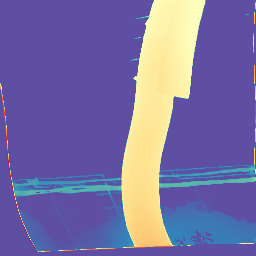
\includegraphics[width=\textwidth]{Collocated_Collage/RS-Homo_depth/RS-Homo/pred_occ068.802_f3921.png}
%     \end{minipage}
%     \begin{minipage}{0.115\textwidth}
%         \vspace{0.05cm}
%         \centering
%         
\includegraphics[width=\textwidth]{Collocated_Collage/RS-Homo_depth/RS-Homo/pred_frame08.png}
%     \end{minipage}
%     \begin{minipage}{0.115\textwidth}
%         \vspace{0.05cm}
%         \centering
%         
\includegraphics[width=\textwidth]{Collocated_Collage/RS-Homo_depth/RS-Homo/pred_frame184.png}
%     \end{minipage}
%     \begin{minipage}{0.115\textwidth}
%         \vspace{0.05cm}
%         \centering
%         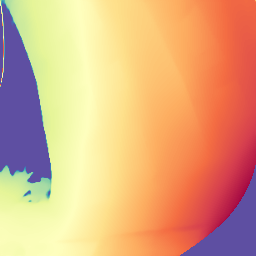
\includegraphics[width=\textwidth]{Collocated_Collage/RS-Homo_depth/RS-Homo/pred_frame958.png}
%     \end{minipage}
%     \begin{minipage}{0.115\textwidth}
%         \vspace{0.05cm}
%         \centering
%         
\includegraphics[width=\textwidth]{Collocated_Collage/RS-Homo_depth/RS-Homo/pred_frame264.png}
%     \end{minipage}
%     \begin{minipage}{0.115\textwidth}
%         \vspace{0.05cm}
%         \centering
%         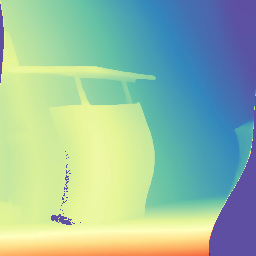
\includegraphics[width=\textwidth]{Collocated_Collage/RS-Homo_depth/RS-Homo/pred_frame96.png}
%     \end{minipage}
%     \begin{minipage}{0.115\textwidth}
%         \vspace{0.05cm}
%         \centering
%         
\includegraphics[width=\textwidth]{Collocated_Collage/RS-Homo_depth/RS-Homo/pred_frame691.png}
%     \end{minipage}
%     \hspace{0.05\textwidth}

%     % RS-Diffusion
%     \begin{minipage}{0.05\textwidth} % Narrow column for row label
%         \raggedleft
%         \rotatebox{90}{\text{RS-D FT \cite{RS-Diffusion}}} % Vertical label for the first row
%     \end{minipage}
%     \begin{minipage}{0.115\textwidth}
%         \vspace{0.05cm}
%         \centering
%         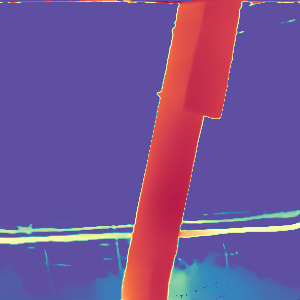
\includegraphics[width=\textwidth]{Collocated_Collage/10-20-vis/rs-diff/occ068.802_f3921 (2).png}
%     \end{minipage}
%     \begin{minipage}{0.115\textwidth}
%         \vspace{0.05cm}
%         \centering
%         
\includegraphics[width=\textwidth]{Collocated_Collage/10-20-vis/rs-diff/frame08.png}
%     \end{minipage}
%     \begin{minipage}{0.115\textwidth}
%         \vspace{0.05cm}
%         \centering
%         
\includegraphics[width=\textwidth]{Collocated_Collage/10-20-vis/rs-diff/frame184.png}
%     \end{minipage}
%     \begin{minipage}{0.115\textwidth}
%         \vspace{0.05cm}
%         \centering
%         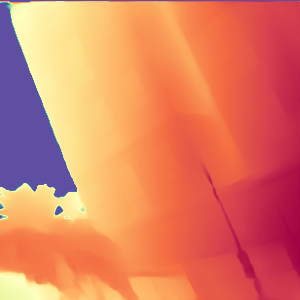
\includegraphics[width=\textwidth]{Collocated_Collage/10-20-vis/rs-diff/frame958.png}
%     \end{minipage}
%     \begin{minipage}{0.115\textwidth}
%         \vspace{0.05cm}
%         \centering
%         
\includegraphics[width=\textwidth]{Collocated_Collage/10-20-vis/rs-diff/frame264.png}
%     \end{minipage}
%     \begin{minipage}{0.115\textwidth}
%         \vspace{0.05cm}
%         \centering
%         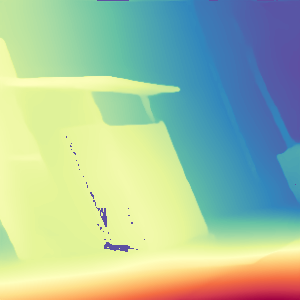
\includegraphics[width=\textwidth]{Collocated_Collage/10-20-vis/rs-diff/frame96.png}
%     \end{minipage}
%     \begin{minipage}{0.115\textwidth}
%         \vspace{0.05cm}
%         \centering
%         
\includegraphics[width=\textwidth]{Collocated_Collage/10-20-vis/rs-diff/frame691.png}
%     \end{minipage}
%     \hspace{0.05\textwidth}

%     % Ours
%     \begin{minipage}{0.05\textwidth} % Narrow column for row label
%         \raggedleft
%         \rotatebox{90}{\text{Ours}} % Vertical label for the first row
%     \end{minipage}
%     \begin{minipage}{0.115\textwidth}
%         \vspace{0.05cm}
%         \centering
%         
\includegraphics[width=\textwidth]{X4K_data/fine_tuned_depth/occ068.802_f3921_pred.png}
%     \end{minipage}
%     \begin{minipage}{0.115\textwidth}
%         % \vspace{0.05cm}
%         \centering
%         
\includegraphics[width=\textwidth]{Collocated_Collage/output_bw_color/frame08.png}
%     \end{minipage}
%     \begin{minipage}{0.115\textwidth}
%         \vspace{0.05cm}
%         \centering
%         
\includegraphics[width=\textwidth]{Collocated_Collage/10-20-vis/output/frame184.png}
%     \end{minipage}
%     \begin{minipage}{0.115\textwidth}
%         \vspace{0.05cm}
%         \centering
%         
\includegraphics[width=\textwidth]{Collocated_Collage/output_bw_color/frame958.png}
%     \end{minipage}
%     \begin{minipage}{0.115\textwidth}
%         \vspace{0.05cm}
%         \centering
%         
\includegraphics[width=\textwidth]{Collocated_Collage/10-20-vis/output/frame264.png}
%     \end{minipage}
%     \begin{minipage}{0.115\textwidth}
%         \vspace{0.05cm}
%         \centering
%         
\includegraphics[width=\textwidth]{Collocated_Collage/output_bw_color/frame96.png}
%     \end{minipage}
%     \begin{minipage}{0.115\textwidth}
%         \vspace{0.05cm}
%         \centering
%         
\includegraphics[width=\textwidth]{Collocated_Collage/10-20-vis/output/frame691.png}
%     \end{minipage}
%     \hspace{0.05\textwidth}

%     % Ground Truth
%     \begin{minipage}{0.05\textwidth} % Narrow column for row label
%         \raggedleft
%         \rotatebox{90}{\text{Ground Truth}} % Vertical label for the first row
%     \end{minipage}
%     \begin{minipage}{0.115\textwidth}
%         % \vspace{0.05cm}
%         \centering
%         
\includegraphics[width=\textwidth]{X4K_data/gt_depth/occ068.802_f3921.png}
%     \end{minipage}
%     \begin{minipage}{0.115\textwidth}
%         \vspace{0.05cm}
%         \centering
%         
\includegraphics[width=\textwidth]{Collocated_Collage/gt_depth_color/frame08.png}
%     \end{minipage}
%     \begin{minipage}{0.115\textwidth}
%         \vspace{0.05cm}
%         \centering
%         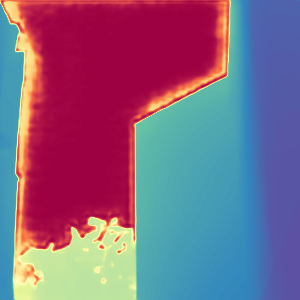
\includegraphics[width=\textwidth]{Collocated_Collage/10-20-vis/gt/frame184.png}
%     \end{minipage}
%     \begin{minipage}{0.115\textwidth}
%         \vspace{0.05cm}
%         \centering
%         
\includegraphics[width=\textwidth]{Collocated_Collage/gt_depth_color/frame958.png}
%     \end{minipage}
%     \begin{minipage}{0.115\textwidth}
%         \vspace{0.05cm}
%         \centering
%         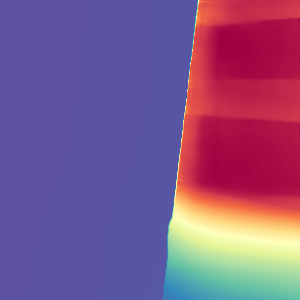
\includegraphics[width=\textwidth]{Collocated_Collage/10-20-vis/gt/frame264.png}
%     \end{minipage}
%     \begin{minipage}{0.115\textwidth}
%         \vspace{0.05cm}
%         \centering
%         
\includegraphics[width=\textwidth]{Collocated_Collage/gt_depth_color/frame96.png}
%     \end{minipage}
%     \begin{minipage}{0.115\textwidth}
%         \vspace{0.05cm}
%         \centering
%         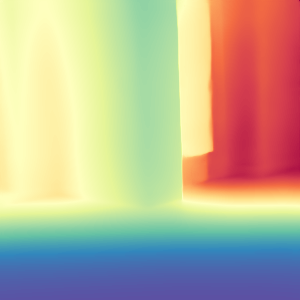
\includegraphics[width=\textwidth]{Collocated_Collage/10-20-vis/gt/frame691.png}
%     \end{minipage}
%     \hspace{0.05\textwidth}

%     \caption{Qualitative results on real scenes. From top to bottom: input image, two baseline comparison outputs, fine-tuned comparison output, our model’s output, and ground truth. Only our method produces accurate depth, demonstrating the two-stage approach preserves scene structure. \textbf{Note Column 5}, where naive affine-based rectification does not work, since the ground truth has a slanted structure. Additional visualizations and comparisons can be seen in the supplementary video.}
%     \label{fig:collocated_results}
%     \vspace{-2mm}
% \end{figure*}

\begin{figure*}
    \centering
    \vspace{0.6in}
    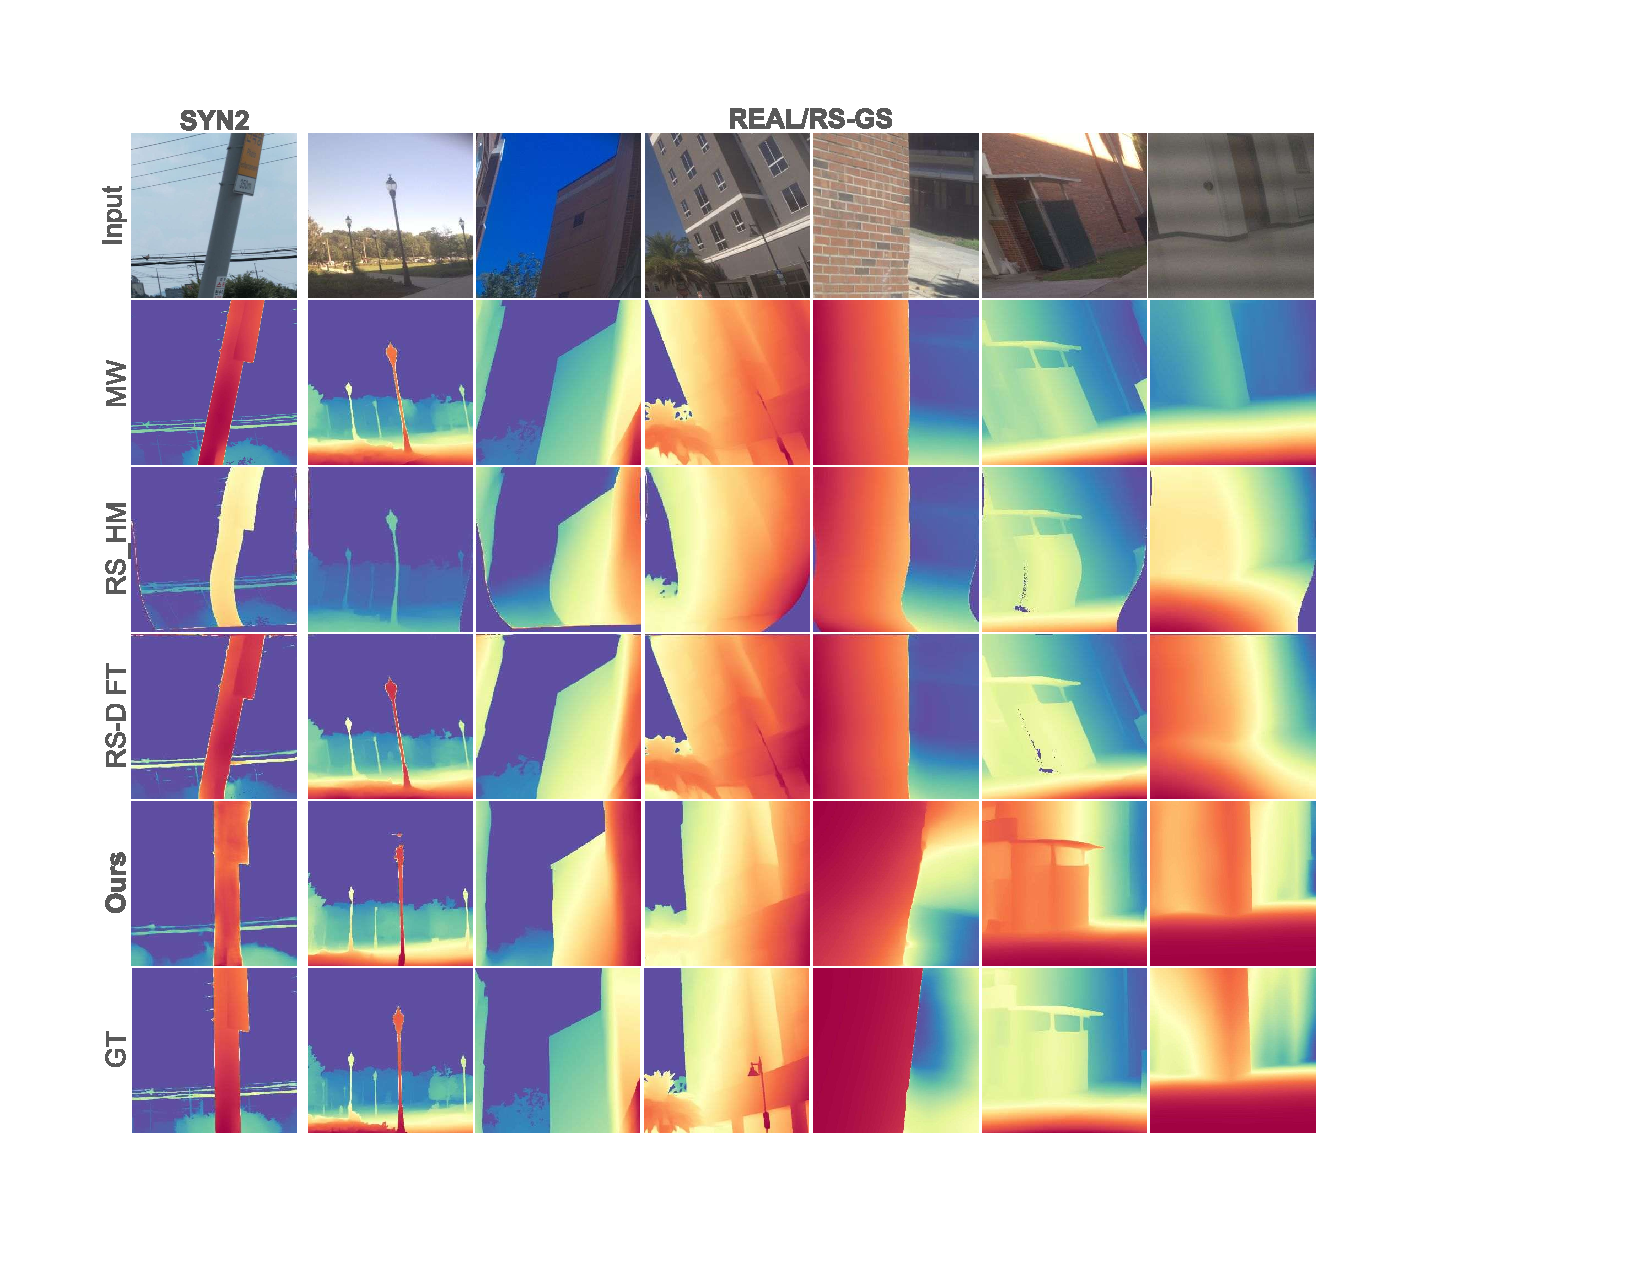
\includegraphics[width=0.8\textwidth, trim={3cm 2.5cm 7cm 3cm}]{Figures/colocated_results.pdf}%
    \vspace{1mm}
    \caption{Qualitative results on real scenes. From top to bottom: input image, two baseline comparison outputs, fine-tuned comparison output, our model’s output, and ground truth. Only our method produces accurate depth, demonstrating the two-stage approach preserves scene structure. \textbf{Note Column 5}, where naive affine-based rectification does not work since the ground truth has a slanted structure. Additional visualizations and comparisons can be seen in the supplementary video.}
    \label{fig:collocated_results}
    % \vspace{-4mm}
\end{figure*}
